%%% -*- coding: utf-8 -*-
\newpage

\chapter{Architecture}
\label{chap:architecture}

The Pucker framework has 4 components: a no limit Texas Hold’em simulation written in JRuby~\cite{jruby.org}, a SQLite storage~\cite{sqlite.org}, a learning and a prediction script written in Python programming language~\cite{python.org}.

The simulation runs the game, inserting data about the states seen by a player and his rewards (or punishments if negative) in the database. The states and rewards are the learning variables. The learning script reads the database, fits the model, and stores the model parameters in disk. The prediction script loads the model and exposes predictions through an HTTP API. The simulation queries the prediction API when a machine learning player needs to take a decision.

\vspace{1cm}
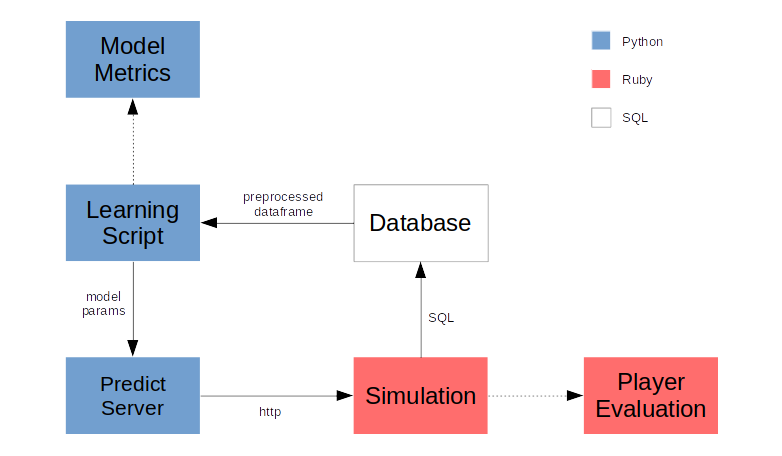
\includegraphics[scale=2]{architecture}

\section{Simulation}
\label{sec:simulation}

The Ruby programming language was chosen to write the simulation component. Ruby offers a great syntax to write game simulations because it is idiomatic, succinct, and object-oriented.

The game of poker, as many other games, is composed of independent reusable components that answer to messages, such as player, dealer and a deck of cards. According to Ampatzoglou and Chatzigeorgiou~\cite{Ampatzoglou2007}, games demand great flexibility, code reusability and low maintenance costs. Consequently, the application of design patterns in them can be beneficial. Ruby is heavily object-oriented and allowed fast development of the simulation.

Due to its idiomacy, the main method of the simulation, the \textit{play} method on the \textit{Game} class, can be understood by anyone. It seems like an english description of the poker game:

\begin{lstlisting}[
    float=h,
    caption=game.rb,
    language=Ruby,
    basicstyle=\tiny\ttfamily,
    commentstyle = \color{gray},
    keywordstyle=\color{red},
    stringstyle=\color{blue},
]
def play
  setup_game
  collect_blinds

  # FLOP
  3.times { deal_table_card }
  bets = collect_bets
  main_pot.merge!(bets)

  # TURN
  deal_table_card
  bets = collect_bets
  main_pot.merge!(bets)

  # RIVER
  deal_table_card
  bets = collect_bets
  main_pot.merge!(bets)

  winners = eligible_players_by_rank
  reward winners

  rotate_and_reset_states
end
\end{lstlisting}

A simple random player can be written in few lines of ruby:

\begin{lstlisting}[
    float=h,
    caption=game.rb,
    language=Ruby,
    basicstyle=\tiny\ttfamily,
    commentstyle = \color{gray},
    keywordstyle=\color{red},
    stringstyle=\color{blue},
]
class DummyPlayer < Player
  def bet(state)
    min_bet = state.min_bet

    choice = rand

    if min_bet > 0 && choice < 1/3.0 # FOLD
      fold
    elsif choice < 2/3.0 # CHECK
      get_from_stack(min_bet)
    else # RAISE
      raise_from(min_bet)
    end
  end
end
\end{lstlisting}

Through the past years, many reusable poker components were written by the Computer Poker Research Group, at the University of Alberta ~\cite{spaz.ca/poker/doc}. Those components were written in the Java programming language. To reuse those components, we chose the JRuby platform to run the poker simulation. This platform runs the Ruby syntax on the Java Virtual Machine~\cite{jruby.org}, and simplifies the calling of Java poker components from Ruby simulation code.

In the context of the Pucker framework, a game has a group of players, a dealer and a pot with the bets of the current game. The dealer deal cards. Players evaluate game state and choose an action based on their current state.

\vspace{1cm}
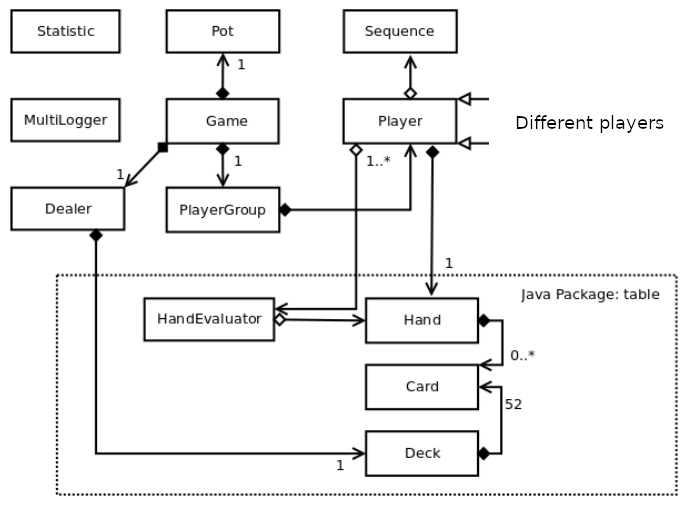
\includegraphics[scale=2]{simulation-diagram}

As previously said (see~\ref{sec:foundations}), Texas Hold'em poker variant has 4 phases: pre-flop, flop, turn and river.

In pre-flop, a player have to take an action with little information about its opponents, since few bets have been committed to the pot. Given that, in pre-flop a player must deal with more imperfect information than in further rounds of the game. Due to its complexity, this research have abstracted the pre-flop phase: every player bets the same as the big-blind player (see~\ref{sec:positions}).

\section{Storage}
\label{sec:storage}

In real poker, there are many game variables, such as how much time a player delayed to take a decision, history of opponent’s decisions, cards on the table, cards in player’s private hand, how strong is the combination of table and hand cards, player position, and many others.

In Pucker, we consider a state as composed by:
\begin{itemize}
  \item Count of players
  \item Count of active players in this round (players who have not folded)
  \item Player's position
  \item Amount in the pot
  \item Amount each player has bet
  \item Number of raises per player
  \item Self amount committed to the pot
  \item Self number of raises
  \item Hand cards
  \item Table cards
  \item Combination of Hand and Table ranking
  \item Combination of Hand and Table strength
  \item Combination of Hand and Table potential
  \item Action taken
\end{itemize}

The reward (or punishment if negative) a player has received in the end of a round is also part of the state. This is the dependent variable our models are trying to predict. Pucker is an extensible framework, it is easy to add or remove variables to the state in future work.

In poker, a player sees a game state, takes an action, and receives a reward (or punishment) in the end of the round. Pucker players remember the states, actions and rewards, and stores them in a SQLite database, one row per action taken.

This is a complex game. To learn a fine strategy, a machine learning player must be fitted from a very large dataset. To accomplish that, the simulation needs to be fast and can't be stopped every round by a slow operation such as database inserts. To overcome this problem, a batch of states are written at once in a single insert query.

\section{Learning}
\label{sec:Learning}

A machine learning prediction typically maps a set of variables to an output. In this work, the input will be the poker state and the output will be the reward seen in the end of this state. In short, the machine learning algorithm will learn to predict the reward, given a state and an action.

To choose the right action, a machine learning player will predict the reward of different actions (fold, call, raise), and choose an action that maximises its rewards. This is inspired in Reinforcement Learning, but without policy optimization~\cite{Silver2016}.

Since the number of states in no limit Texas Hold’em is $10^{160}$~\cite{Johanson2013}, it is impossible to store every state. It is even hard to store the number of states to take a good decision. To overcome this, we will store only the model parameters and erase the database of states after the learning process.

It is crucial for the model to be extensible: it may correct its parameters according to new data, it will not be able to access the full history. Neural Networks are naturally capable of incremental learning, and this is a big reason of their choice in favor of other models, like Gradient Boosting Machines. According to~\cite{xgboost-github}, until today popular Gradient Boosting Machine implementations cannot handle inclemental learning.

Instead of considering the game round (pre-flop, flop, turn or river) a variable of the state, past work~\cite{Sirin2008} and ~\cite{Moravcik2017} has seen better results by creating a separate model for different rounds, and we will also consider that. The main reason is that different rounds of poker are played in very different ways because they have a different state. Additionally, the number of possible states in poker is huge~\cite{Johanson2013}, by using different models in different rounds we are reducing the number of possible states a model has to learn from.

The learning component is a Python script that reads states from a database, preprocess, fits a prediction model and stores its parameters in disk.

\subsection{Neural Networks Architectures}

\subsection{Bayesian Networks and Initial Dataset}
\label{sec:data-generation}

In order to train a supervised model, it is needed a dataset. The performance of a machine learning model relies heavily on the quality of this dataset~\cite{Polikar2001}. A realiable dataset must represent reality with confidence, thus it should be generated from real situations.

In Pucker, after the models are trained, new datasets can be generated from subsequential games played by those models. But still remains the problem of how to generate a initial dataset with good quality.

Untrained Neural Networks could be put to play. Since their parameters are not fitted yet, they will play randomly according to the random generation of its initial parameters. The quality of this dataset is worse than a dataset generated from good players, because it represents random situations, hardly seen in professional games.

Pucker Framework introduces a initial set of simple players that are put to play against each other. Rather than playing randomly, those players use Bayesian Networks~\cite{Heckerman1998} to analyse state and choose better poker actions. To certify that Bayesian players perform better, they were put to play against random players and won by a large margin in the long run. They were also tested against "always check" players, and won by a large margin.

Bayesian networks are tree structures that represent conditional dependencies of variables in a directed acyclic graph, and are capable of infere from those variables~\cite{Neapolitan2003}.

Nodes of this graph represents Bayesian variables. In poker, those nodes can represent the poker state: hand ranking, number of players, position, etc. Unconnected nodes represent variables that are conditionally independent of each other, like a player hand and position. Nodes are associated with a probability function that represents the chance of possible states of that node. Edges represent conditional dependencies, for example, a good poker hand depends on the private player hand and the public table cards.

After some experiments, two different architectures were chosen to compose poker players in order to generate a initial dataset. The first one in simpler, and relies only on the state minimum bet and hand rank. The second uses players' position, together with minimum bet, to compose a scenario conditional variable. When the Bayesian Network detects a high winning condition, bayesian players raise. When it detects a low winning condition, bayesian players check. If it's a losing condition, it folds, or checks if minimum bet is zero.

As an example, the bayesian player represented by figure~\ref{fig:simple-bn} will fold with a bad hand when there is a minimum bet over zero. And it will re-raise when it has a great hand and the minimum bet is over zero.

\begin{figure}[H]
  \centering
  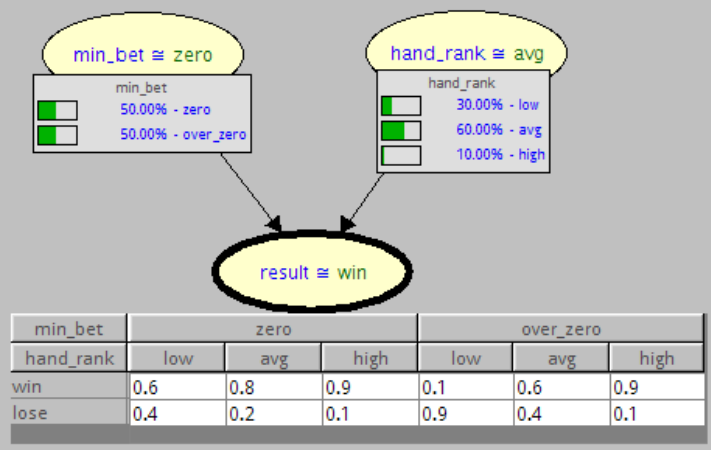
\includegraphics[width=1\textwidth]{simple_bn}
  \caption{Simple bayesian network with its probabilities}
  \label{fig:simple-bn}
\end{figure}

\begin{figure}[H]
  \centering
  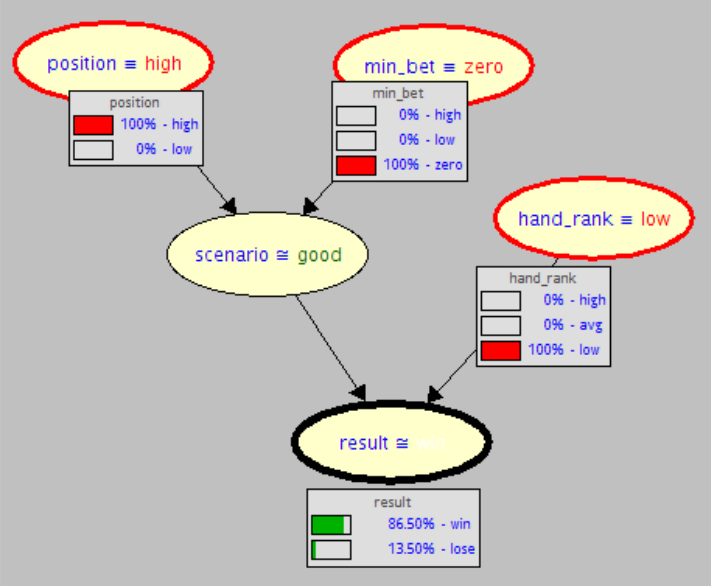
\includegraphics[width=1\textwidth]{best_bn}
  \caption{Better bayesian network. It is represented a situation of high position, zero bets and low hand rank. This player might bluff in this situation.}
\end{figure}
\vspace{0.5cm}

Those two bayesian networks played 40000 games in a five players Texas Hold'em table. This table also had a random player to generate diverse situations in order to generalize the initial dataset. The result is a 566739 row database that was used to train the initial neural networks. After that, the neural networks played against each other, generated even better quality datasets, and learned incrementally from their self-plays.


\section{Prediction}
\label{sec:prediction}

The prediction component is trivial. It reads the stored model parameters and creates an instance of the model ready to predict from new states.

There are two problems: this is a slow process, and the Ruby simulation cannot run Python code seamlessly, as they are different languages running in different virtual machines. To overcome those problems, the prediction component keeps an instance of the model in memory and exposes an HTTP API that receives a state and returns a prediction.

This component is capable of exposing many different models, one per HTTP endpoint. This way, Pucker supports the simulation of many different machine learning algorithms playing at the same time.

To build the HTTP API, Pucker uses the Flask library~\cite{flask.pocoo.org}.

%%% Local Variables:
%%% mode: latex
%%% TeX-master: thesis.tex
%%% End:
